\documentclass[11pt,a4paper]{article}

% ---------------------------------------------------------------------------
% Overleaf-ready. Compile with pdfLaTeX. Upload this file plus the six PNGs
% (crossing.png, prep_sweep.png, step.png, life_lost.png, bias_by_prep.png,
% contexts.png) either flat or in a figures/ folder -- both paths are set.
% ---------------------------------------------------------------------------

\usepackage[margin=2.5cm]{geometry}
\usepackage{amsmath,amssymb,amsthm}
\usepackage{booktabs}
\usepackage{graphicx}
\usepackage{enumitem}
\usepackage{caption}
\usepackage{xcolor}
\definecolor{linkblue}{RGB}{25,60,130}
\usepackage[colorlinks=true,linkcolor=linkblue,citecolor=linkblue,urlcolor=linkblue]{hyperref}
\captionsetup{font=small,labelfont=bf}

\graphicspath{{figures/}{./}}

\newtheorem{proposition}{Proposition}
\newtheorem{lemma}{Lemma}
\newtheorem{corollary}{Corollary}
\theoremstyle{remark}
\newtheorem{remark}{Remark}
\newtheorem{assumption}{Assumption}

\newcommand{\dd}{\,\mathrm{d}}
\newcommand{\cface}{c_{\mathrm{f}}}
\newcommand{\pderiv}[2]{\frac{\partial #1}{\partial #2}}

\title{An optimal-stopping model for the timing of social transition}
\author{Madeline}
\date{September 2026}

\begin{document}
\maketitle

\begin{abstract}
The decision of when to socially transition is formulated as a deterministic optimal-stopping problem. The decision-maker balances an increasing marginal cost of continuing to present as their assigned sex against a decreasing marginal cost of being socially transitioned and read as transgender. The second cost is driven by a clock probability that combines several independent cues multiplicatively, only one of which is hormone-gated. First- and second-order conditions are derived, a sufficient condition for uniqueness of the interior optimum is given, and step discontinuities in the switching cost at context-formation dates are shown to relocate the optimum to the step under a weak condition. Analytic sensitivities of the optimum to every parameter are obtained by the implicit function theorem and verified numerically. Four qualitative results follow: the optimum is a vector with one entry per social context; non-hormonal preparation has increasing returns and advances the optimum; any weighting that respects the irreversibility of time collapses the optimum toward the present; and bias in self-perception of the face is second-order while other cues dominate but first-order once they are removed. The model has no predictive power over the numerical value of the optimum. Its content is the sign of each partial derivative.
\end{abstract}

% ===========================================================================
\section{Introduction}
% ===========================================================================

A person beginning gender-affirming hormone therapy (HRT) faces a timing problem. Physical change is slow and partly outside their control; the cost of continuing to present as their assigned sex is immediate and, for many, rising; and the cost of presenting as their affirmed gender before they are reliably read as such depends on where they are and who is looking. Informal reasoning about this problem tends to collapse it to a single question, ``when will I pass?'', and to treat the answer as the date on which social transition becomes viable.

This note argues that the informal framing is structurally wrong in three ways, and that a simple model makes the errors visible. First, the cost of waiting is not constant: the literature on concealment shows it to be cognitively and affectively taxing in a way that compounds \cite{pachankis2007,testa2015}. Second, the decision is not one decision: the relevant environment differs by context, and the empirical evidence on chosen-name use is explicitly per-context \cite{russell2018}. Third, the physical variables most relevant to being read as female in a brief encounter are largely not the ones HRT changes: facial hair, brow shape and voice are unaffected or barely affected by oestrogen \cite{hembree2017,davies2015}, and are disproportionately influential in gender categorisation of faces and voices \cite{brown1993,gelfer2005}.

The contribution is a compact optimal-stopping formulation in which each of these points appears as a term whose effect on the optimum can be signed analytically. Section~\ref{sec:background} reviews the relevant physiology, perception and psychology literature. Section~\ref{sec:method} sets up the model and its numerical implementation. Section~\ref{sec:results} derives the optimality conditions, the effect of switching-cost discontinuities, the sensitivities and the per-context structure. Section~\ref{sec:discussion} interprets the results, records corrections to an earlier version of the analysis, and states the limitations. Section~\ref{sec:conclusion} concludes.

% ===========================================================================
\section{Background}
\label{sec:background}
% ===========================================================================

\subsection{Physiological timelines under feminising hormone therapy}

The Endocrine Society clinical practice guideline \cite{hembree2017} tabulates expected effects of feminising therapy with onset and time-to-maximum. Body-fat redistribution has an expected onset of 3--6 months and a maximum effect at 2--5 years; skin softening and decreased oiliness at 3--6 months; decreased terminal-hair growth at 6--12 months with maximum beyond 3 years. The guideline states explicitly that oestrogen does not remove existing terminal facial hair, and that voice is unaffected. The WPATH Standards of Care \cite{coleman2022} are consistent with this. These timelines motivate the sigmoidal face-cue function of \S\ref{sec:clock}: no visible facial change for the first few months, most of the achievable change over the following two to three years, and a floor set by bone structure that hormones cannot move.

\subsection{Cues in gender categorisation}

Rapid gender categorisation of faces is driven disproportionately by a small number of features. In a feature-isolation and feature-substitution experiment, Brown and Perrett \cite{brown1993} found that brows and eyes carried the most gender information when viewed in isolation, and that the jaw, brows-and-eyes, chin and brows produced the largest change in perceived gender when grafted between male and female prototypes. Bruce et al.\ \cite{bruce1993} reached compatible conclusions with a different paradigm, and Campbell et al.\ \cite{campbell1999} showed that brow position alone shifts gender attribution. For voice, Gelfer and Mikos \cite{gelfer2005} found that fundamental frequency and formant frequencies each contribute to gender identification from isolated vowels, and Davies, Papp and Antoni \cite{davies2015} review the evidence that oestrogen does not alter the adult voice and that voice feminisation is achieved through training or surgery.

Two modelling consequences follow. Brows, facial hair and voice deserve to be separate cues, because they are separately influential and separately controllable. And they are not hormone-gated, so their contribution to the clock probability is a function of preparation effort rather than of time on HRT.

\subsection{The cost of concealment and the cost of visibility}

Meyer's minority-stress framework \cite{meyer2003} distinguishes distal stressors (discrimination, rejection, victimisation) from proximal stressors: expectations of rejection, concealment, and internalised stigma. Testa et al.\ \cite{testa2015} adapt the framework to transgender and gender-nonconforming populations and include \emph{nondisclosure} and \emph{negative expectations for future events} as measured proximal stressors. Pachankis \cite{pachankis2007} gives a cognitive--affective--behavioural process model of concealing a stigma in which vigilance, preoccupation and the threat of discovery accumulate rather than habituate. In the model of \S\ref{sec:method}, the boymoding cost $B(t)$ corresponds to the proximal stressors of concealment and nondisclosure, and the visible-trans cost $A\,C(t)$ to the distal stressors weighted by the probability of being identified.

\subsection{Social transition and mental-health outcomes}

Durwood, McLaughlin and Olson \cite{durwood2017} report that socially transitioned transgender children have depression and self-worth scores comparable to cisgender controls. Russell et al.\ \cite{russell2018}, in a sample of 129 transgender youth, find that chosen-name use is associated with lower depression, suicidal ideation and suicidal behaviour, with the association strengthening as the number of contexts in which the chosen name can be used increases. The per-context structure of that finding is the empirical motivation for treating the optimum as a vector in \S\ref{sec:contexts}.

\subsection{Optimal stopping}

The problem is a deterministic optimal-stopping problem: choose a time $\tau$ to move from one cost regime to another, paying a switching cost. The economics of irreversible investment under uncertainty \cite{dixit1994} provides the natural comparison; the stochastic version of the present problem would carry an option value of waiting in exactly that sense. The present model is deterministic and so omits option value; this is discussed in \S\ref{sec:limits}.

% ===========================================================================
\section{Methodology}
\label{sec:method}
% ===========================================================================

\subsection{Setup and notation}

Let $t\ge 0$ denote time in months since the start of HRT and let $T$ be a planning horizon. The decision variable is a switching time $\tau\in[0,T]$: before $\tau$ the decision-maker presents as their assigned sex; from $\tau$ onward they are socially transitioned. Three cost streams are defined on $[0,T]$ in a common unit of disutility per month.

\paragraph{Boymoding cost.}
\begin{equation}
  B(t) = B_0\,(1+\beta t), \qquad B_0>0,\ \beta\ge 0. \label{eq:B}
\end{equation}
The growth rate $\beta$ encodes the accumulating character of concealment stress \cite{pachankis2007}. Setting $\beta=0$ recovers the informal model.

\paragraph{Life-lost term.}
\begin{equation}
  \ell(t) = \ell_0\,e^{-\lambda t}, \qquad \ell_0\ge 0,\ \lambda>0. \label{eq:ell}
\end{equation}
This is the marginal value of authentic time forgone while boymoding. It is an opportunity cost of an irreversible resource rather than a rate of discomfort, and it is decreasing to reflect that early time is scarcer.

\paragraph{Visible-trans cost.}
\begin{equation}
  V(t;r) = A\,C(t;r), \label{eq:V}
\end{equation}
where $A>0$ is a context-hostility coefficient and $C(t;r)\in[0,1]$ is the probability of being read as transgender in a brief encounter, defined in \S\ref{sec:clock}.

\paragraph{Switching cost.}
\begin{equation}
  S(\tau) = s_0 + \sum_j \Delta_j\, H(\tau - t_j), \qquad \Delta_j>0, \label{eq:S}
\end{equation}
with $H$ the right-continuous Heaviside function. Introducing oneself into a context on the day $t_j$ it forms costs $s_0$; re-introducing oneself afterwards costs an additional $\Delta_j$.

\subsection{Clock probability}
\label{sec:clock}

\begin{assumption}[Independent cues]\label{ass:indep}
A person is read as transgender if any one of a set of cues $\mathcal{I}$ fires, and the cues fire independently.
\end{assumption}

Under Assumption~\ref{ass:indep},
\begin{equation}
  C(t;r) = 1 - \prod_{i\in\mathcal{I}}\bigl(1-c_i(t;r)\bigr) =: 1 - \Pi(t;r), \label{eq:C}
\end{equation}
where $c_i$ is the probability that cue $i$ alone produces a clock and $\Pi$ is the survival product. Following \S\ref{sec:background}, $\mathcal{I}=\{\mathrm{face},\mathrm{hair},\mathrm{brow},\mathrm{voice}\}$.

\paragraph{Face cue (hormone-gated).}
\begin{equation}
  \cface(t) = c_\infty + (c_0-c_\infty)\,\sigma\!\bigl(-k(t-t_h)\bigr), \qquad \sigma(x)=\tfrac{1}{1+e^{-x}}, \label{eq:cface}
\end{equation}
where $c_0$ is the pre-treatment asymptote ($t\to-\infty$), $c_\infty$ the floor set by bone structure, $k$ the rate of change and $t_h$ the month of half-maximal change. Note that $\cface(0)<c_0$: at the defaults of Table~\ref{tab:params}, $\cface(0)=0.671$. Its derivative is
\begin{equation}
  \cface'(t) = -(c_0-c_\infty)\,k\,\sigma(-k(t-t_h))\bigl[1-\sigma(-k(t-t_h))\bigr]\le 0. \label{eq:dcface}
\end{equation}

\paragraph{Non-hormonal cues.} For $i\in\{\mathrm{hair},\mathrm{brow},\mathrm{voice}\}$,
\begin{equation}
  c_i(r) = c_i^0\,(1-e_i r), \qquad c_i^0,\,e_i\in[0,1], \label{eq:ci}
\end{equation}
with $r\in[0,1]$ a preparation fraction and $e_i$ the share of the cue removable at full preparation. These cues do not depend on $t$ \cite{hembree2017,davies2015}.

\begin{lemma}[Derivatives of the clock probability]\label{lem:dC}
\begin{align}
  \pderiv{C}{r} &= -\Pi\sum_{i\ne\mathrm{f}}\frac{c_i^0 e_i}{1-c_i(r)} \le 0, \label{eq:dCdr}\\
  \pderiv{C}{t} &= \Pi\,\frac{\cface'(t)}{1-\cface(t)} \le 0, \label{eq:dCdt}\\
  \pderiv{C}{\cface} &= \frac{\Pi}{1-\cface} = \prod_{i\ne\mathrm{f}}\bigl(1-c_i(r)\bigr) \ge 0. \label{eq:dCdcf}
\end{align}
\end{lemma}
\begin{proof}
From $\ln\Pi=\sum_i\ln(1-c_i)$, $\partial_x\Pi = \Pi\sum_i\frac{-\partial_x c_i}{1-c_i}$ for any argument $x$. For $x=r$, $\partial_r c_i=-c_i^0 e_i$ on the non-hormonal cues and $0$ on the face. For $x=t$ only the face term is non-zero. For $x=\cface$ the sum has the single term $-1/(1-\cface)$. Then $C=1-\Pi$.
\end{proof}

\subsection{Objective}

The total cost of switching at $\tau$ is
\begin{equation}
  J(\tau) = \int_0^{\tau}\bigl[B(t)+\ell(t)\bigr]\dd t + \int_{\tau}^{T} A\,C(t;r)\dd t + S(\tau). \label{eq:J}
\end{equation}
Define the marginal gap
\begin{equation}
  g(t) := B(t)+\ell(t)-A\,C(t;r). \label{eq:g}
\end{equation}
A negative $g$ means the marginal cost of switching now exceeds the marginal cost of waiting one more month.

\subsection{Numerical implementation and parameters}
\label{sec:numerics}

The model is implemented in Python (package \texttt{transition\_timing}). The interior root of $g$ is found by Brent's method; the global minimiser of $J$ is obtained by evaluating \eqref{eq:J} by adaptive quadrature at the interior root, at the endpoints, and at the left limit of every step in $S$. Every analytic derivative in this note is checked against a central finite difference: \eqref{eq:dCdr} and \eqref{eq:dCdt} to relative error $10^{-8}$, $g'$ to $10^{-7}$, and the sensitivities of \S\ref{sec:sens} to $10^{-4}$. A test suite of 25 cases covers limits, monotonicity, the derivative identities, the step result of Proposition~\ref{prop:step}, and the sign of every entry of Table~\ref{tab:sens}.

Default parameters are in Table~\ref{tab:params}. The face-cue timeline is set from \cite{hembree2017}: negligible change in the first three months, half of the achievable change by month 16, and most of it by month 36. The relative sizes of $c^0_{\mathrm{voice}}>c^0_{\mathrm{hair}}>c^0_{\mathrm{brow}}$ follow the ordering of cue strength in \cite{brown1993,gelfer2005} but the absolute values are judgement. The remaining parameters ($B_0,\beta,A,r,\ell_0$) are unobservable and chosen to give a shallow interior crossing so that the sensitivities are legible.

\begin{table}[t]
  \centering
  \caption{Default parameters. Every parameter except the face timeline is a judgement, not an estimate.}
  \label{tab:params}
  \begin{tabular}{llr}
    \toprule
    symbol & meaning & value \\
    \midrule
    $B_0$ & baseline boymoding cost & 0.55 \\
    $\beta$ & growth rate of boymoding cost & 0.03 \\
    $\ell_0,\ \lambda$ & life-lost amplitude, decay & 0,\ 0.03 \\
    $A$ & context hostility & 0.80 \\
    $r$ & preparation fraction & 0.15 \\
    $c_0,\ c_\infty$ & face cue: pre-treatment asymptote, floor & 0.70,\ 0.15 \\
    $k,\ t_h$ & face cue: rate, half-way month & 0.18,\ 16 \\
    $(c^0,e)_{\mathrm{hair}}$ & hair cue: untreated probability, efficacy & (0.60,\ 0.85) \\
    $(c^0,e)_{\mathrm{brow}}$ & brow cue & (0.40,\ 0.85) \\
    $(c^0,e)_{\mathrm{voice}}$ & voice cue & (0.75,\ 0.80) \\
    $T$ & horizon, months & 36 \\
    \bottomrule
  \end{tabular}
\end{table}

% ===========================================================================
\section{Results}
\label{sec:results}
% ===========================================================================

\subsection{Optimality conditions}

\begin{proposition}[First-order condition]\label{prop:foc}
On any interval on which $S$ is differentiable, a stationary point $\tau^*$ of $J$ satisfies
\begin{equation}
  B(\tau^*)+\ell(\tau^*)+S'(\tau^*) = A\,C(\tau^*;r). \label{eq:foc}
\end{equation}
Between steps, where $S'=0$, this is $g(\tau^*)=0$.
\end{proposition}
\begin{proof}
By the Leibniz rule, $J'(\tau)=B(\tau)+\ell(\tau)-A\,C(\tau;r)+S'(\tau)$.
\end{proof}

\begin{proposition}[Second-order condition and uniqueness]\label{prop:soc}
Between steps, $J''(\tau)=g'(\tau)$ with
\begin{equation}
  g'(t) = B_0\beta - \lambda\,\ell(t) - A\,\pderiv{C}{t}(t;r). \label{eq:gprime}
\end{equation}
An interior root $\tau^*$ of $g$ is a strict local minimum of $J$ if
\begin{equation}
  B_0\beta + A\Bigl|\pderiv{C}{t}(\tau^*;r)\Bigr| > \lambda\,\ell_0 e^{-\lambda\tau^*}, \label{eq:soc}
\end{equation}
and if \eqref{eq:soc} holds on all of $[0,T]$ then $g$ is strictly increasing and the root is unique.
\end{proposition}
\begin{proof}
Differentiate \eqref{eq:g} using \eqref{eq:B}, \eqref{eq:ell} and \eqref{eq:dCdt}; the first and third terms of \eqref{eq:gprime} are non-negative and the second non-positive. Strict monotonicity gives uniqueness.
\end{proof}

With $\ell_0=0$, \eqref{eq:soc} holds whenever $\beta>0$ or $C$ is strictly decreasing. At the defaults, $\min_{[0,36]}g'=0.0167>0$ and the interior optimum is $\tau^*=12.63$ months (Figure~\ref{fig:crossing}). Boundary cases: $g(0)\ge 0$ gives $\tau^*=0$; $g(T)<0$ means no crossing within the horizon.

\begin{figure}[t]
  \centering
  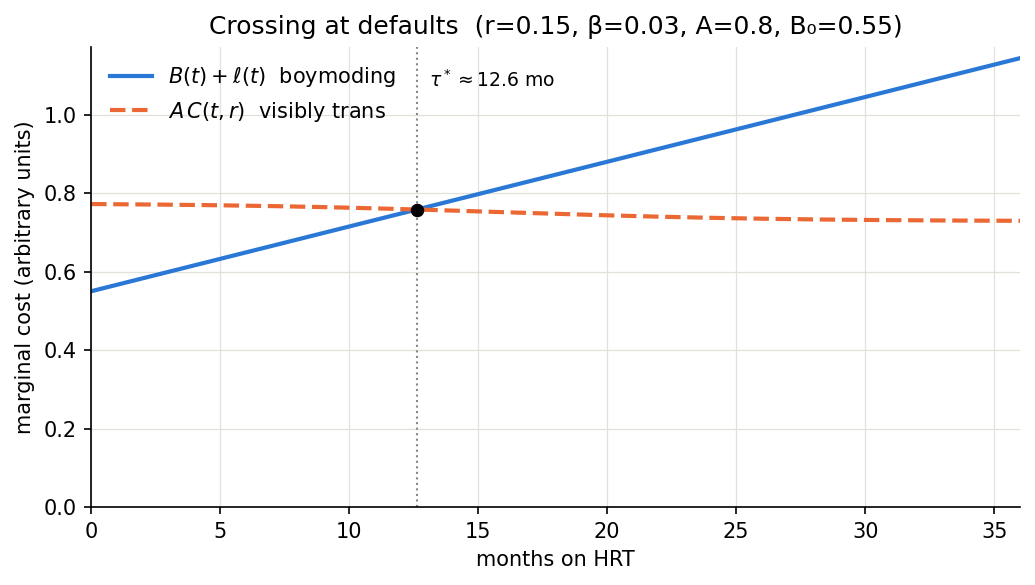
\includegraphics[width=0.85\textwidth]{crossing}
  \caption{Marginal cost streams at the default parameters. The interior optimum is the crossing.}
  \label{fig:crossing}
\end{figure}

\subsection{Step discontinuities at context formation}
\label{sec:step}

Let $J_0$ be the objective with $S\equiv s_0$ and let $\tau_s$ be its interior minimiser. Add one step of height $\Delta$ at a context-formation date $t_c<\tau_s$.

\begin{proposition}[Relocation to the step]\label{prop:step}
With $J(\tau)=J_0(\tau)+\Delta\,H(\tau-t_c)$, the global minimiser is
\begin{equation}
  \tau^* = \begin{cases} t_c^- & \Delta>\Delta^* := J_0(t_c)-J_0(\tau_s),\\ \tau_s & \text{otherwise,}\end{cases}
  \qquad\text{with}\qquad
  \Delta^* = \int_{t_c}^{\tau_s}\bigl(-g(t)\bigr)\dd t. \label{eq:deltastar}
\end{equation}
\end{proposition}
\begin{proof}
On $[0,t_c)$, $J=J_0$ and $J_0'=g<0$, so the infimum over the interval is $J_0(t_c)$, approached from the left. On $[t_c,T]$, $J=J_0+\Delta$, minimised at $\tau_s$ by uniqueness. Compare. The integral form follows from $J_0(t_c)-J_0(\tau_s)=-\int_{t_c}^{\tau_s}J_0'$.
\end{proof}

\begin{corollary}\label{cor:shallow}
$\Delta^*$ is bounded by $(\tau_s-t_c)\,|g(t_c)|$, and is small whenever the crossing is shallow. In that regime the smooth-model penalty for switching early is second-order and a modest re-introduction cost relocates the optimum.
\end{corollary}

At the defaults with $t_c=1$: $\Delta^*=1.21$, equal to $2.20$ months of $B_0$. Figure~\ref{fig:step} shows $J(\tau)$ for four values of $\Delta$; at $\Delta=2$ the optimum has moved from $12.6$ to $1.0$.

\begin{figure}[t]
  \centering
  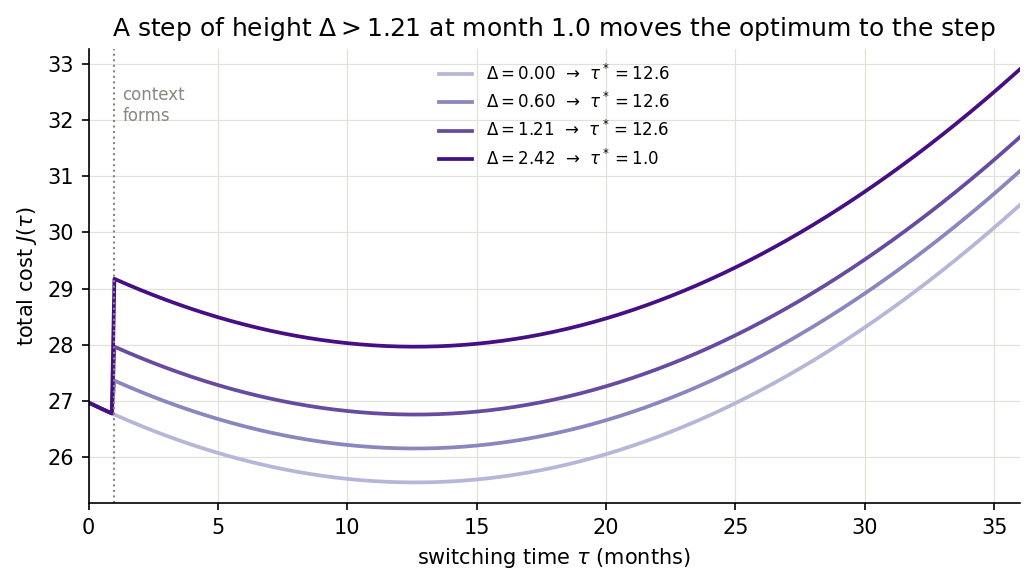
\includegraphics[width=0.85\textwidth]{step}
  \caption{$J(\tau)$ with a step of height $\Delta$ at month 1. For $\Delta>\Delta^*=1.21$ the optimum is at the step.}
  \label{fig:step}
\end{figure}

\subsection{Sensitivity of the interior optimum}
\label{sec:sens}

For any parameter $\theta$, the implicit function theorem applied to $g(\tau^*;\theta)=0$ gives
\begin{equation}
  \pderiv{\tau^*}{\theta} = -\frac{\partial g/\partial\theta}{\partial g/\partial\tau}\bigg|_{\tau^*}, \label{eq:ift}
\end{equation}
and since $g'(\tau^*)>0$, the sign of $\partial\tau^*/\partial\theta$ is opposite to that of $\partial g/\partial\theta$. Table~\ref{tab:sens} lists every partial with its value at the defaults and a finite-difference check.

\begin{table}[t]
  \centering
  \caption{Sensitivities of $\tau^*$ at the defaults ($\tau^*=12.63$). Units: months per unit of $\theta$.}
  \label{tab:sens}
  \begin{tabular}{llrrr}
    \toprule
    $\theta$ & $\partial g/\partial\theta$ & sign & analytic & finite diff. \\
    \midrule
    $r$ & $-A\,\partial_r C>0$ & $-$ & $-7.60$ & $-7.60$ \\
    $\beta$ & $B_0\tau^*>0$ & $-$ & $-377$ & $-377$ \\
    $B_0$ & $1+\beta\tau^*>0$ & $-$ & $-74.9$ & --- \\
    $\ell_0$ & $e^{-\lambda\tau^*}>0$ & $-$ & $-37.2$ & --- \\
    $A$ & $-C(\tau^*)<0$ & $+$ & $+51.5$ & $+51.5$ \\
    $\cface$ & $-A\prod_{i\ne\mathrm{f}}(1-c_i)<0$ & $+$ & $+4.58$ & --- \\
    \bottomrule
  \end{tabular}
\end{table}

\paragraph{Growth rate.} $\partial\tau^*/\partial\beta=-377$: raising $\beta$ from $0.03$ to $0.04$ advances the optimum by nearly four months. Because $g$ is shallow near its root, small changes in the slope of $B$ move the root far. Models with $\beta=0$ therefore systematically overstate $\tau^*$.

\paragraph{Preparation has increasing returns.} From \eqref{eq:dCdr}, $|\partial_r C|\propto\Pi$, and $\Pi$ itself grows as $r$ removes cues. Numerically $-\partial\tau^*/\partial r$ rises from $7.6$ at $r=0.15$ to $15.6$ at $r=1$ (Table~\ref{tab:biasr}, Figure~\ref{fig:prep}). Under Assumption~\ref{ass:indep}, each surviving cue caps the benefit of removing the others, so the last cue removed is worth more than the first.

\paragraph{Life-lost weighting.} Ordinary discounting weights future cost less and biases stopping models toward delay. The irreversibility of youth argues the opposite weighting. With $\ell_0=0.2$ the optimum moves from $12.6$ to $2.0$ months; with $\ell_0\ge 0.3$ it is $\tau^*=0$ (Figure~\ref{fig:lifelost}).

\begin{figure}[t]
  \centering
  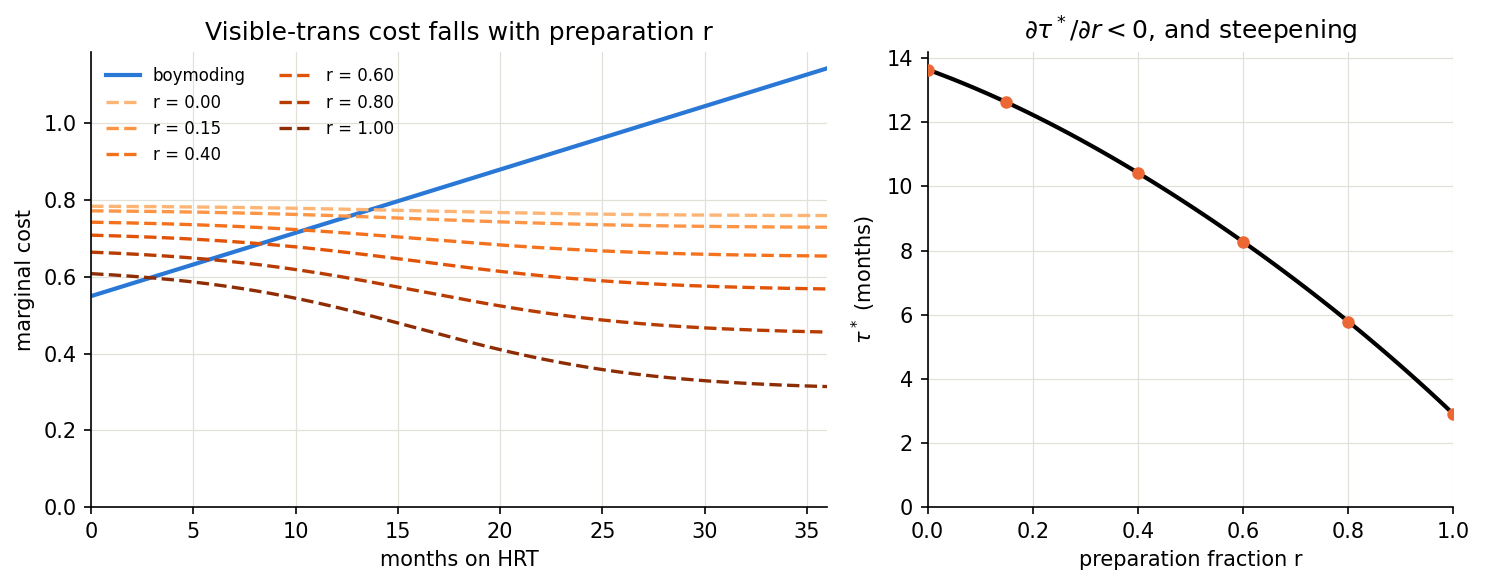
\includegraphics[width=\textwidth]{prep_sweep}
  \caption{Left: visible-trans cost for several $r$. Right: $\tau^*(r)$, convex, reflecting increasing returns.}
  \label{fig:prep}
\end{figure}

\begin{figure}[t]
  \centering
  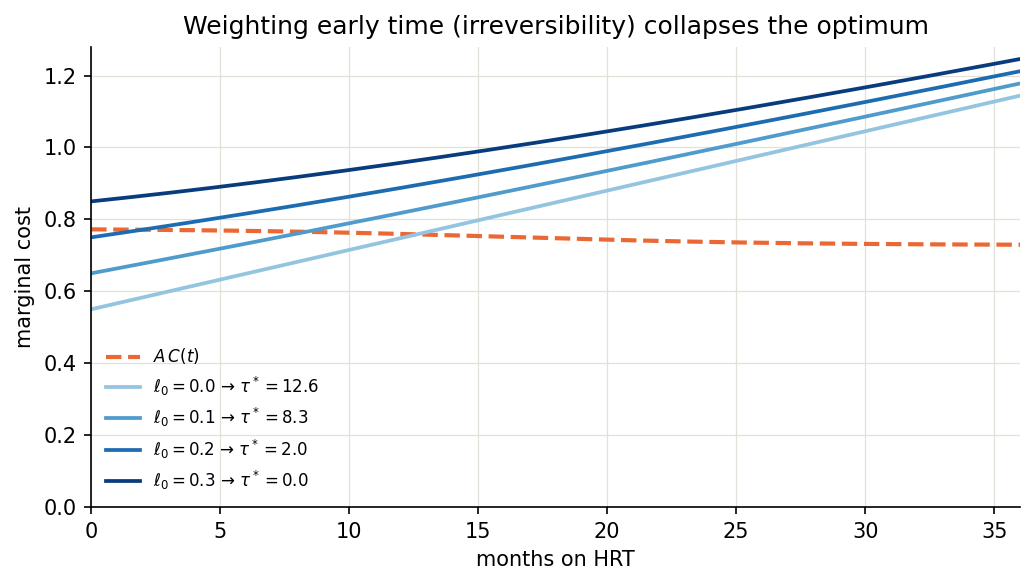
\includegraphics[width=0.85\textwidth]{life_lost}
  \caption{Adding $\ell(t)$ to the boymoding cost. Each curve is labelled with the resulting $\tau^*$.}
  \label{fig:lifelost}
\end{figure}

\subsection{Bias in self-perception}
\label{sec:bias}

\begin{assumption}[Pessimistic self-perception]\label{ass:bias}
The decision-maker's estimate of their own face cue is $\hat\cface=\cface+b$ with $b>0$.
\end{assumption}

Assumption~\ref{ass:bias} is stated as an assumption rather than a cited fact. The general unreliability of self-perception of appearance is well documented; the pessimistic direction is specific to dysphoria and is not claimed here beyond the modelling assumption.

From Table~\ref{tab:sens}, $\partial\tau^*/\partial\cface>0$: pessimistic bias delays the perceived optimum. The magnitude is
\begin{equation}
  \pderiv{\tau^*}{\cface} = \frac{A}{g'(\tau^*)}\prod_{i\ne\mathrm{f}}\bigl(1-c_i(r)\bigr), \label{eq:biassens}
\end{equation}
by \eqref{eq:dCdcf} and \eqref{eq:ift}. The product is the probability that no non-face cue fires. When preparation is low it is small and the face cannot change the decision much, because the person will be clocked on voice or hair regardless. When preparation is complete it is near one and every unit of perceived $\cface$ moves $\tau^*$ directly.

\begin{table}[t]
  \centering
  \caption{Both sensitivities as functions of preparation $r$.}
  \label{tab:biasr}
  \begin{tabular}{rrr}
    \toprule
    $r$ & $\partial\tau^*/\partial\cface$ & $-\partial\tau^*/\partial r$ \\
    \midrule
    0.15 & 4.58 & 7.60 \\
    0.40 & 8.76 & 9.93 \\
    0.60 & 13.27 & 11.57 \\
    0.80 & 19.30 & 13.35 \\
    1.00 & 27.64 & 15.64 \\
    \bottomrule
  \end{tabular}
\end{table}

Table~\ref{tab:biasr} and Figure~\ref{fig:bias} give the numbers. At $r=0.15$ a bias $b=0.10$ delays $\tau^*$ by $0.45$ months; at $r=0.8$ the same bias delays it by $1.87$ months ($5.79\to7.66$). The cross-partial $\partial^2\tau^*/\partial\cface\,\partial r$ is positive throughout.

\begin{figure}[t]
  \centering
  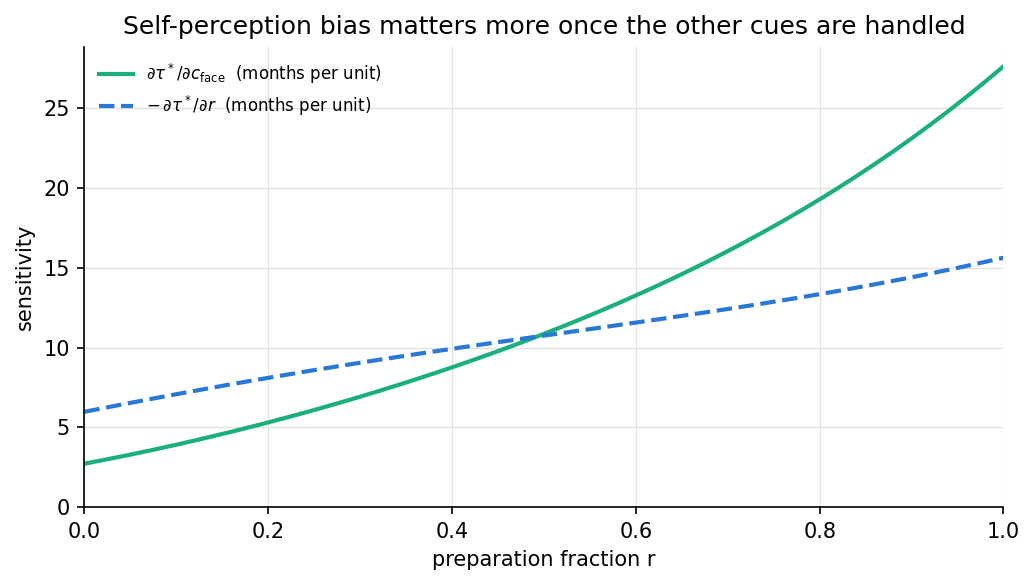
\includegraphics[width=0.85\textwidth]{bias_by_prep}
  \caption{Both sensitivities grow with $r$; the face-perception sensitivity grows faster because it is proportional to the survival product of the other cues, \eqref{eq:biassens}.}
  \label{fig:bias}
\end{figure}

\subsection{The optimum is a vector}
\label{sec:contexts}

$A$ and $S$ are properties of a context, not of the decision-maker. With contexts indexed by $j$,
\begin{equation}
  J(\boldsymbol\tau) = \sum_j\Biggl[\int_0^{\tau_j}\bigl[B_j+\ell_j\bigr]\dd t + \int_{\tau_j}^T A_j\,C(t;r)\dd t + S_j(\tau_j)\Biggr], \label{eq:Jvec}
\end{equation}
which is separable when contexts do not interact, so each $\tau_j^*$ solves its own copy of \eqref{eq:foc}. Solving for a single $\tau^*$ with a pooled $A$ optimises for the most hostile context and applies that answer everywhere. This is the modelling counterpart of the per-context finding of \cite{russell2018}.

At the defaults with three illustrative contexts (Figure~\ref{fig:ctx}): a newly forming context with $A=0.45$ and a step $\Delta=1.5$ at month 1 gives $\tau^*=0$; a general urban context with $A=0.80$ gives $12.6$; a high-hostility context with $A=1.20$ gives $33.1$.

\begin{figure}[t]
  \centering
  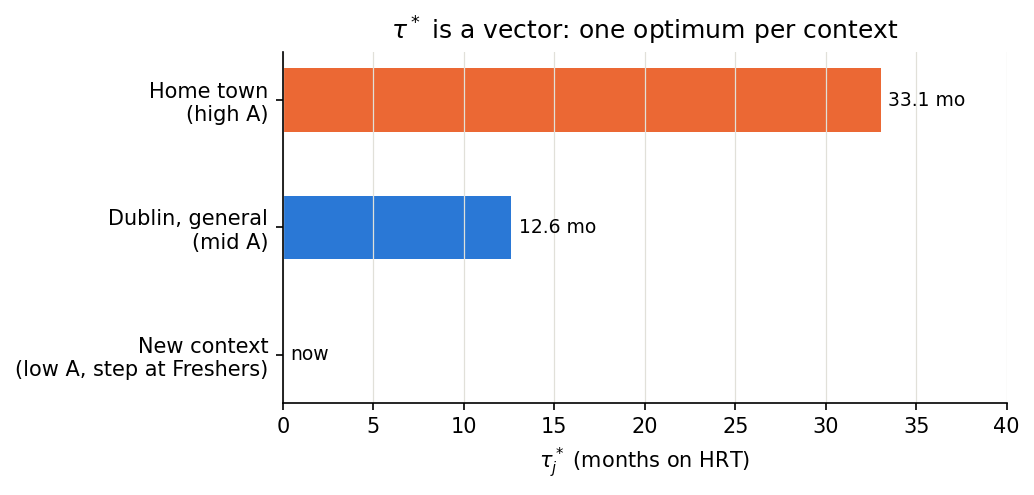
\includegraphics[width=0.75\textwidth]{contexts}
  \caption{Per-context optima at the defaults.}
  \label{fig:ctx}
\end{figure}

% ===========================================================================
\section{Discussion}
\label{sec:discussion}
% ===========================================================================

\subsection{Interpretation}

The results share a direction. Every mechanism that the informal ``when will I pass'' framing leaves out (the growth of concealment cost, the irreversibility of time, the step in switching cost at context formation, the per-context structure of hostility, and the non-hormonal cues) moves the optimum earlier than that framing implies. The only parameters that delay it are hostility $A$ and pessimistic self-perception, and the second of these is shown in \S\ref{sec:bias} to be second-order until the non-hormonal cues are handled.

The increasing-returns result of \S\ref{sec:sens} has a practical reading. Under the multiplicative structure, effort on the largest surviving cue has the highest marginal value, and for a person early in HRT the largest cues are precisely those HRT does not touch. The cross-partial of \S\ref{sec:bias} has a related reading: calibrating self-perception (controlled monthly photographs, external feedback) becomes decision-relevant only once preparation is advanced, and is wasted effort before.

\subsection{Corrections to an earlier version}

Three errors in an earlier informal version of this analysis are recorded here.
\begin{enumerate}[nosep]
  \item The first-order condition was written as $B=A\,C+S'$. The correct form is \eqref{eq:foc}, $B+\ell+S'=A\,C$. The sign of $S'$ was reversed. The error was harmless for piecewise-constant $S$ but is corrected.
  \item Self-perception bias was described as propagating ``straight through'' to a late optimum. Section~\ref{sec:bias} shows this to be true only at high $r$; at the default $r=0.15$ the effect is small. The exact dependence is \eqref{eq:biassens}.
  \item $c_0$ was described as the face-only clock probability at $t=0$. It is the pre-treatment asymptote; $\cface(0)=0.671$ at the defaults.
\end{enumerate}

\subsection{Limitations}
\label{sec:limits}

\paragraph{No number.} Every parameter in Table~\ref{tab:params} except the face timeline is unobservable. Figure~\ref{fig:prep} shows $\tau^*$ ranging from $0$ to beyond the horizon across plausible values. The model is not identified and should not be used to compute a date. Its content is the sign of each entry of Table~\ref{tab:sens}, and those signs are robust to any reparametrisation preserving $B$ non-decreasing and $C$ non-increasing in $t$ and decreasing in $r$.

\paragraph{Deterministic.} A stochastic version would carry an option value of waiting in the sense of \cite{dixit1994}: information about how $\cface$ evolves arrives over time. This argues for delay, against the irreversibility of $\ell$. Neither is quantified here.

\paragraph{Independence.} Assumption~\ref{ass:indep} is a first approximation. Gender categorisation involves configural as well as featural processing \cite{brown1993}, so cues interact. Positive interaction (cues reinforcing one another) would strengthen the increasing-returns result; negative interaction would weaken it.

\paragraph{One switch per context.} Real transition is a set of partial, reversible, separately timed changes within each context. The vector formulation captures the context dimension but not the within-context ordering.

\paragraph{Cost of visibility only.} The model has no positive term for authentic time independent of being clocked. $\ell$ is a partial proxy. A fuller model would move $\tau^*$ earlier still.

% ===========================================================================
\section{Conclusion}
\label{sec:conclusion}
% ===========================================================================

A deterministic optimal-stopping model of social-transition timing has been set up, solved, and its sensitivities signed analytically and verified numerically. The model's numerical output is not informative. Its structural output is: the concealment cost grows and its growth rate dominates the optimum; non-hormonal preparation advances the optimum with increasing returns; irreversibility of time collapses the optimum toward the present; switching-cost steps at context formation relocate the optimum to the step under a weak condition; the optimum is a vector, one entry per context; and pessimistic self-perception is second-order until the non-hormonal cues are removed. Each of these is a claim about the sign of a derivative, and each is robust to the choice of parameters.

% ===========================================================================
\begin{thebibliography}{99}
\setlength{\itemsep}{2pt}

\bibitem{hembree2017}
W.~C. Hembree, P.~T. Cohen-Kettenis, L.~Gooren, S.~E. Hannema, W.~J. Meyer, M.~H. Murad, S.~M. Rosenthal, J.~D. Safer, V.~Tangpricha, and G.~G. T'Sjoen.
Endocrine treatment of gender-dysphoric/gender-incongruent persons: an Endocrine Society clinical practice guideline.
\emph{Journal of Clinical Endocrinology \& Metabolism}, 102(11):3869--3903, 2017.
\href{https://doi.org/10.1210/jc.2017-01658}{doi:10.1210/jc.2017-01658}.

\bibitem{coleman2022}
E.~Coleman, A.~E. Radix, W.~P. Bouman, et al.
Standards of Care for the Health of Transgender and Gender Diverse People, Version~8.
\emph{International Journal of Transgender Health}, 23(S1):S1--S259, 2022.
\href{https://doi.org/10.1080/26895269.2022.2100644}{doi:10.1080/26895269.2022.2100644}.

\bibitem{davies2015}
S.~Davies, V.~G. Papp, and C.~Antoni.
Voice and communication change for gender nonconforming individuals: giving voice to the person inside.
\emph{International Journal of Transgenderism}, 16(3):117--159, 2015.
\href{https://doi.org/10.1080/15532739.2015.1075931}{doi:10.1080/15532739.2015.1075931}.

\bibitem{gelfer2005}
M.~P. Gelfer and V.~A. Mikos.
The relative contributions of speaking fundamental frequency and formant frequencies to gender identification based on isolated vowels.
\emph{Journal of Voice}, 19(4):544--554, 2005.
\href{https://doi.org/10.1016/j.jvoice.2004.10.006}{doi:10.1016/j.jvoice.2004.10.006}.

\bibitem{brown1993}
E.~Brown and D.~I. Perrett.
What gives a face its gender?
\emph{Perception}, 22(7):829--840, 1993.
\href{https://doi.org/10.1068/p220829}{doi:10.1068/p220829}.

\bibitem{bruce1993}
V.~Bruce, A.~M. Burton, E.~Hanna, P.~Healey, O.~Mason, A.~Coombes, R.~Fright, and A.~Linney.
Sex discrimination: how do we tell the difference between male and female faces?
\emph{Perception}, 22(2):131--152, 1993.
\href{https://doi.org/10.1068/p220131}{doi:10.1068/p220131}.

\bibitem{campbell1999}
R.~Campbell, P.~J. Benson, S.~B. Wallace, S.~Doesbergh, and M.~Coleman.
More about brows: how poses that change brow position affect perceptions of gender.
\emph{Perception}, 28(4):489--504, 1999.
\href{https://doi.org/10.1068/p2784}{doi:10.1068/p2784}.

\bibitem{meyer2003}
I.~H. Meyer.
Prejudice, social stress, and mental health in lesbian, gay, and bisexual populations: conceptual issues and research evidence.
\emph{Psychological Bulletin}, 129(5):674--697, 2003.
\href{https://doi.org/10.1037/0033-2909.129.5.674}{doi:10.1037/0033-2909.129.5.674}.

\bibitem{testa2015}
R.~J. Testa, J.~Habarth, J.~Peta, K.~Balsam, and W.~Bockting.
Development of the Gender Minority Stress and Resilience Measure.
\emph{Psychology of Sexual Orientation and Gender Diversity}, 2(1):65--77, 2015.
\href{https://doi.org/10.1037/sgd0000081}{doi:10.1037/sgd0000081}.

\bibitem{pachankis2007}
J.~E. Pachankis.
The psychological implications of concealing a stigma: a cognitive--affective--behavioral model.
\emph{Psychological Bulletin}, 133(2):328--345, 2007.
\href{https://doi.org/10.1037/0033-2909.133.2.328}{doi:10.1037/0033-2909.133.2.328}.

\bibitem{russell2018}
S.~T. Russell, A.~M. Pollitt, G.~Li, and A.~H. Grossman.
Chosen name use is linked to reduced depressive symptoms, suicidal ideation, and suicidal behavior among transgender youth.
\emph{Journal of Adolescent Health}, 63(4):503--505, 2018.
\href{https://doi.org/10.1016/j.jadohealth.2018.02.003}{doi:10.1016/j.jadohealth.2018.02.003}.

\bibitem{durwood2017}
L.~Durwood, K.~A. McLaughlin, and K.~R. Olson.
Mental health and self-worth in socially transitioned transgender youth.
\emph{Journal of the American Academy of Child \& Adolescent Psychiatry}, 56(2):116--123, 2017.
\href{https://doi.org/10.1016/j.jaac.2016.10.016}{doi:10.1016/j.jaac.2016.10.016}.

\bibitem{dixit1994}
A.~K. Dixit and R.~S. Pindyck.
\emph{Investment Under Uncertainty}.
Princeton University Press, 1994.

\end{thebibliography}

\end{document}
